\documentclass{article}
\usepackage[utf8]{inputenc}
\usepackage[T1]{fontenc}
\usepackage{amsmath}
\usepackage{amsfonts}
\usepackage{subcaption}
\usepackage{graphicx}
\graphicspath{ {./img/} }
\usepackage{float}
\usepackage{listings}
\usepackage{pdfpages}
\usepackage{babel}
\usepackage[scaled]{helvet}
\usepackage{hyperref}
\usepackage{fancyhdr}
\usepackage{color}
\usepackage{url}
\usepackage{xcolor}
\usepackage{tabularx}
\usepackage{array}
\usepackage{longtable}
\usepackage{multirow,makecell}
\usepackage{indentfirst}
\usepackage{bold-extra}
\usepackage{lmodern}
\usepackage{amssymb} 
\usepackage{geometry}

\geometry{hmargin=2.5cm,vmargin=2.5cm}

\setcellgapes{1pt}
\makegapedcells
\newcolumntype{R}[1]{>{\raggedleft\arraybackslash }b{#1}}
\newcolumntype{L}[1]{>{\raggedright\arraybackslash }b{#1}}
\newcolumntype{C}[1]{>{\centering\arraybackslash }b{#1}}

%%%%%%%%%%%%%%%% Lengths %%%%%%%%%%%%%%%%
\setlength{\textwidth}{15.5cm}
\setlength{\evensidemargin}{0.5cm}
\setlength{\oddsidemargin}{0.5cm}

\lstset{ keywordstyle=\color{blue},
         stringstyle=\color{red},
         commentstyle=\color{green},
         morecomment=[l][\color{magenta}]{\#},
         basicstyle=\ttfamily,
         breaklines=false,
         keywords=[2]{void,int,float,double,T,size_t,bool,unsigned,long,mipp_fonction,type, type1,type2, uint_type, float, uint, float32_t, float64_t, int8_t, int16_t, int32_t, int64_t, uint8_t, uint16_t, uint32_t, uint64_t},
         keywords=[3]{lmul},
         keywords=[4]{msk, rvm_float32_m2_t},
         keywords=[5]{reg, rvd_float32_m2_t},
         keywords=[6]{const},
         keywords=[7]{mipp_function},
         keywords=[8]{masque, maskedoff},
         keywordstyle={[2]\ttfamily\color{blue!90!black}},
         keywordstyle={[3]\ttfamily\color{purple!50!blue}},
         keywordstyle={[4]\ttfamily\color{blue!30!orange}},
         keywordstyle={[5]\ttfamily\color{green!60!blue}},
         keywordstyle={[6]\ttfamily\color{red}},
         keywordstyle={[7]\ttfamily\color{orange}},
         keywordstyle={[8]\ttfamily\color{gray}}
}


%================NEWCOMMAND=====================

\newcommand{\mipp}{MIPPv2\ }
\newcommand{\ti}[1]{\texttt{#1}}
\newcommand{\tic}[2]{\texttt{\textbf{\textcolor{#1}{#2}}}}

%===============================================

\begin{document}



\newlength{\larg}
\setlength{\larg}{15.5cm}
 
% La commande \title... bien chargée ! 
\title{
\vspace{1cm}
{\rule{\larg}{1mm}}\vspace{7mm}
\begin{tabular}{p{4cm} r}
   & {\Huge {\bf Documentation MIPP v2}} \\
   & \\
   & {\huge Extension vectorielle RISC-V}
\end{tabular}\\
\vspace{2mm}
{\rule{\larg}{1mm}}
\vspace{2mm} \\



\centering 

\includegraphics[width=7cm]{img/riscv.png}\\

\includegraphics[width=10cm]{img/mipp.jpg} 


\vspace{4.0cm}

}

\author{\begin{tabular}{p{13.7cm}}
Edgar Baucher
\end{tabular}\\
\hline }
\date{}
 
\maketitle

\section{L’extension vectorielle de RISC-V}

L'architecture RISC-V possède une structure et un jeu d'instruction qui se montre sur certains points fondamentalement différent des autres jeux d'instructions. Sur l'extension vectorielle, la plus singulière des différences est certainement l'utilisation du LMUL:

\subsection{LMUL (vector \textbf{L}ength \textbf{MUL}tiplier)}

   Le LMUL est un nombre pouvant prendre les valeurs : \texttt{1/8, 1/4, 1/2, 1, 2, 4} ou \texttt{8}. Il fait partie intégrante de la configuration d'un registre vectoriel dans le language assembleur, c'est à dire que le nombre d'éléments dans un tel registre dépend seulement de 3 choses: 
\begin{itemize}
	\item La taille des registres vectoriels simple (déterminée par le matériel).
	\item Le type des éléments contenu dans le vecteur.
	\item La valeur du LMUL.
\end{itemize}

Sa fonctionnalité quand il est inférieur à 1 est légèrement différente par rapport aux autres valeurs, mais sa logique reste la même.

\subsubsection{LMUL>=1}

Lorsque le LMUL est supérieur ou égal à 1, sa valeur désigne le nombre de registres vectoriels groupés qui vont former le vecteur final. Soit SEW le nombre de bits sur lequel est matériellement codé un registre vectoriel, au bas niveau, lors de la configuration d'un registre vectoriel en assembleur, au lieu de réserver SEW bits, la machine va réserver $SEW\times LMUL$ bits pour le vecteur. C'est à dire que tous les registres vectoriels matériels groupés doivent être placés sur une mémoire contigüe. Ainsi, les registres vectoriels des jeux d'instructions plus classiques sont des registres vectoriels configuré avec LMUL=1. Un exemple avec LMUL=2 est illustré en figure \ref{fig:LMUL}, où les r$i$, $i\in \{0, nombreRegistresVectoriels-1\}$ représentent les registres vectoriels matériels.\\


\begin{figure}[H]
    \centering
    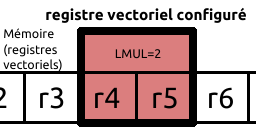
\includegraphics[width=0.4\linewidth]{img/LMUL.png}
    \caption{Exemple avec LMUL=2}
    \label{fig:LMUL}
\end{figure}


Cette fonctionnalité trouve son utilité dans l'optimisation de performances. En effet, une fois qu'un registre vectoriel est configuré avec un LMUL>1, effectuer une opération sur ce vecteur ne prendra qu'une seule instruction assembleur, ce qui permet de vectoriser jusqu'à 8 fois plus de données qu'une vectorisation classique. 



\subsubsection{LMUL<1}

Puis, quand le LMUL est inférieur à 1, au lieu de grouper des vecteurs, il divise le vecteur: en configurant le registre vectoriel avec LMUL = 1/2, il n'y a que la moitié du registre vectoriel matériel qui est utilisée pour remplir les données et faire les opérations.\\

Le nombre d'applications de cette fonctionnalité étant relativement restreint, elle n'a pas été inclue à MIPP, il n'est possible que d'utiliser des LMUL supérieurs ou égaux à 1.

\subsection{Taille agnostique des registres vectoriels}

   Un autre particularité de l'extension vectorielle du RISC-V est sa gestion agnostique des registres vectoriels lors de la compilation. Ce comportement est aussi utilisé par SVE, son utilité est de former un exécutable mobile (pouvant être exécuté par un processeur différent du moment qu'il possède le même jeu d'instruction), mais cela provoque un gros défaut pour les programmeurs: la taille des registres vectoriels n'est pas accessible au moment de la compilation. Le seul moyen de l'obtenir est de l'appeler au moment de l'exécution, ce qui rend tout de suite la vie plus difficile pour les développeurs de librairies SIMD (Single Instruction Multiple Data).\\

La première raison à cela est la difficulté de manier un type de registre vectoriel. Comme la taille de l'objet n'est pas connue à la compilation, en C/C++, un tel type est considéré comme un \ti{sizeless struct}. Avec les versions actuelle des compilateurs, cette structure ne peut faire office d'attribut d'une classe ou d'une structure, et la notion d'adressage n'est absolument pas sécurisée car l'objet est physiquement situé au niveau du processeur et non de la RAM. Les seules actions réalisables sont l'utilisation en fonction (passage en argument, type de retour ou recours aux intrinsèques), ou le renommage du type avec un \tic{blue}{typedef}.\\
   
La deuxième raison concerne MIPP, qui est un wrapper, or, les wrapper ne peuvent pas stocker de variables. Il est donc impossible de récupérer la taille des registres vectoriel au début du programme pour ensuite la réutiliser.\\

\subsection{Fonctions intrinsèques vectorielles}

   Structure syntaxique 

\section{Wrapper de vectorisation: MIPP v2}

\subsection{Implémentation en 3 couches}
   
   C, C++, C++ avec classe\\
   un mipp\_v2\_impl\_RVV.h qui crée les fonctions C à partir des intrinsèques C propres au processeu\\
   un mipp.h qui s'occupe de faire les LMUL=1 par défaut\\
   un mipp.hpp qui s’occupe de faire les fonctions c++ à partir des fonctions c\\

\subsection{Gestion des vecteurs à taille agnostique}

   type comme champ d'une classe (géré par mipp.hpp)

\subsection{Utilisation}

   \subsubsection{Types}

      
Pour l'interface moyen niveau C++, la déclaration d'un registre vectoriel ou d'un masque se fait par l'utilisation des templates:

\begin{center}
\begin{tabular}{c}
\begin{lstlisting}
reg<type, lmul> r;
msk<type, lmul> m;
\end{lstlisting}
\end{tabular}
\end{center}

Où les types et les valeur de \texttt{lmul} possible sont listées dans ce tableau:

\begin{center}
\begin{tabular}{|l|p{8cm}|} 
   \hline \texttt{\color{blue}type} & \texttt{int8\_t, int16\_t, int32\_t, int64\_t (int), uint8\_t, uint16\_t, uint32\_t, uint64\_t (unsinged int), float32\_t (float), float64\_t (double)}\\
   \hline \texttt{\color{purple}LMUL} & \texttt{1, 2, 4, 8,  $\varnothing$}\\
   \hline
\end{tabular}
\end{center}

En revanche, les templates n'existant pas en C, les noms des types dans \mipp bas niveau sont le résultat de l'application d'un \tic{blue}{typedef} sur un nom de type explicite. Ils prennent cette syntaxe :
\begin{center}
\begin{longtable}{l l}

Registre vectoriel: & \ti{rvd\_\textcolor{blue}{\textbf{type}}\_m\textcolor{purple}{\textbf{LMUL}}\_t}\\
Masque: & \ti{rvm\_\textcolor{blue}{\textbf{type}}\_m\textcolor{purple}{\textbf{LMUL}}\_t}\\

\end{longtable}
\end{center}

Où \tic{blue}{type} et \tic{purple}{LMUL} peuvent prendre les valeurs:

\begin{center}
\begin{tabular}{|l|p{8cm}|} 
   \hline \texttt{\textbf{\color{blue}type}} & \texttt{int8, int16, int32, int64, uint8, uint16, uint32, uint64, float32, float64}\\
   \hline \texttt{\textbf{\color{purple}LMUL}} & \texttt{1, 2, 4, 8}\\
   \hline
\end{tabular}
\end{center}

Afin d'épargner la gestion et compréhension du \ti{LMUL} aux utilisateurs qui n'en n'ont pas besoin, il est possible dans les deux interfaces \mipp de ne pas indiquer de \ti{LMUL}, qui aura pour valeur par défaut \ti{LMUL=1}. Ce qui donne ces syntaxes de type possible: 

\begin{center}
\begin{tabular}{|l|c|c|}
\hline & Moyen niveau (\ti{C++}) & Bas niveau (\ti{C})\\

\hline Registre vectoriel
&
\begin{lstlisting}
   reg<type>
\end{lstlisting}
&
\ti{rvd\_\textcolor{blue}{\textbf{type}}\_t}
\\
\hline Masque
&
\begin{lstlisting}
   msk<type>
\end{lstlisting}
&
\ti{rvm\_\textcolor{blue}{\textbf{type}}\_t}
\\ \hline   
\end{tabular}
\end{center}

   \subsubsection{Fonctions}
   
      Dans la liste de prototypes C++ qui va suivre, les * indiquent que le rôle fonction est détaillé dans l'explication \ref{it:expl}.

\begin{center}
\setlength{\LTleft}{-20cm plus -1fill}
\setlength{\LTright}{\LTleft}
\small
\begin{longtable}{l r}

\begin{lstlisting}
    int  N<type, lmul> N()
\end{lstlisting} & MIPP N*\\
\begin{lstlisting}
    void load(const type* addr, reg<type,lmul>& r)
\end{lstlisting} & load*\\
\begin{lstlisting}
    void loadu(const type* addr, reg<type,lmul>& r)
\end{lstlisting} & unaligned load*\\
\begin{lstlisting}
    void cmask(const type* addr, reg<type,lmul>& r)
\end{lstlisting} &  cmask*\\
\begin{lstlisting}
    void store(const type* addr, reg<type,lmul> r)
\end{lstlisting} & store*\\
\begin{lstlisting}
    void set(reg<type,lmul>& r, type scalar)
\end{lstlisting} & set\\
\begin{lstlisting}
    void set1(reg<type,lmul>& r, type scalar)
\end{lstlisting} & set\\
\begin{lstlisting}
    void set1(msk<type, lmul>& r, bool scalar)
\end{lstlisting} & set for mask\\
\begin{lstlisting}
    void set0(reg<type,lmul>& r)
\end{lstlisting} & fill with 0\\
\begin{lstlisting}
    void set0(msk<type, lmul>& r)
\end{lstlisting} & fill with 0\\
\begin{lstlisting}
    reg<type,lmul> add(reg<type,lmul> r1, reg<type,lmul> r2)
\end{lstlisting} & r1+r2\\
\begin{lstlisting}
    reg<type,lmul> sub(reg<type,lmul> r1, reg<type,lmul> r2)
\end{lstlisting} & r1-r2\\
\begin{lstlisting}
    reg<type,lmul> mul(reg<type,lmul> r1, reg<type,lmul> r2)
\end{lstlisting} & r1*r2\\
\begin{lstlisting}
    reg<type,lmul> div(reg<type,lmul> r1, reg<type,lmul> r2)
\end{lstlisting} & r1/r2\\
\begin{lstlisting}
    reg<type,lmul> min(reg<type,lmul> r1, reg<type,lmul> r2)
\end{lstlisting} & min\\
\begin{lstlisting}
    reg<type,lmul> max(reg<type,lmul> r1, reg<type,lmul> r2)
\end{lstlisting} & max\\
\begin{lstlisting}
    reg<type,lmul> andb(reg<type,lmul> r1, reg<type,lmul> r2)
\end{lstlisting} & r1\&r2*\\
\begin{lstlisting}
    msk<type, lmul> andb(msk<type, lmul> r1, msk<type, lmul> r2)
\end{lstlisting} & r1 \&\& r2*\\
\begin{lstlisting}
    reg<type,lmul> orb(reg<type,lmul> r1, reg<type,lmul> r2)
\end{lstlisting} & r1 | r2\\
\begin{lstlisting}
    msk<type, lmul> orb(msk<type, lmul> r1, msk<type, lmul> r2)
\end{lstlisting} & r1 || r2\\
\begin{lstlisting}
    reg<type,lmul> xorb(reg<type,lmul> r1, reg<type,lmul> r2)
\end{lstlisting} & r1 $\hat{ }$ r2\\
\begin{lstlisting}
    msk<type, lmul> xorb(msk<type, lmul> r1, msk<type, lmul> r2)
\end{lstlisting} & (r1 \tiny{\&\&} \small !r2)  || (!r1 \tiny{\&\&} \small r2)\\
\begin{lstlisting}
    reg<type,lmul> andnb(reg<type,lmul> r1, reg<type,lmul> r2)
\end{lstlisting} & (!r1)\&r2\\
\begin{lstlisting}
    msk<type, lmul> andnb(msk<type, lmul> r1, msk<type, lmul> r2)
\end{lstlisting} & !r1 \&\& r2\\
\begin{lstlisting}
    reg<type,lmul> lshiftr(reg<type,lmul> r1, reg<type,lmul> r2)
\end{lstlisting} & r1<<r2*\\
\begin{lstlisting}
    reg<type,lmul> rshiftr(reg<type,lmul> r1, reg<type,lmul> r2)
\end{lstlisting} & r1>>r2\\
\begin{lstlisting}
    reg<type,lmul> lshift(reg<type,lmul> r1, type scalar)
\end{lstlisting} & r1<<scalar\\
\begin{lstlisting}
    reg<type,lmul> rshift(reg<type,lmul> r1, type scalar)
\end{lstlisting} & r1>>scalar\\
\begin{lstlisting}
    reg<type,lmul> blend(reg<type,lmul> r1, reg<type,lmul> r2, msk<type, lmul> m)
\end{lstlisting} & blend*\\
\begin{lstlisting}
    reg<type,lmul> sat(reg<type,lmul> r1, type min, type max)
\end{lstlisting} & saturate*\\
\begin{lstlisting}
    reg<type,lmul> fmadd(reg<type,lmul> r1, reg<type,lmul> r2, reg<type,lmul> r3)
\end{lstlisting} & (r1*r2)+r3\\
\begin{lstlisting}
    reg<type,lmul> fnmadd(reg<type,lmul> r1, reg<type,lmul> r2, reg<type,lmul> r3)
\end{lstlisting} & -(r1*r2)+r3\\
\begin{lstlisting}
    reg<type,lmul> fmsac(reg<type,lmul> r1, reg<type,lmul> r2, reg<type,lmul> r3)
\end{lstlisting} & (r2*r3)-r1\\
\begin{lstlisting}
    reg<type,lmul> fnmsac(reg<type,lmul> r1, reg<type,lmul> r2, reg<type,lmul> r3)
\end{lstlisting} & -(r2*r3)+r1\\
\begin{lstlisting}
    reg<type,lmul> fmacc(reg<type,lmul> r1, reg<type,lmul> r2, reg<type,lmul> r3)
\end{lstlisting} & (r2*r3)+r1\\
\begin{lstlisting}
    reg<type,lmul> fnmacc(reg<type,lmul> r1, reg<type,lmul> r2, reg<type,lmul> r3)
\end{lstlisting} & -(r2*r3)-r1\\
\begin{lstlisting}
    reg<type,lmul> sqrt(reg<type,lmul> r)
\end{lstlisting} & $\sqrt{r}$\\
\begin{lstlisting}
    reg<type,lmul> rsqrt(reg<type,lmul> r)
\end{lstlisting} & 1/$\sqrt{r}$\\
\begin{lstlisting}
    reg<type,lmul> notb(reg<type,lmul> r)
\end{lstlisting} & binar NOT\\
\begin{lstlisting}
    msk<type, lmul> notb(msk<type, lmul> r1)
\end{lstlisting} & !r\\
\begin{lstlisting}
    reg<type,lmul> neg(reg<type,lmul> r)
\end{lstlisting} & -r\\
\begin{lstlisting}
    msk<type, lmul> cmpeq(reg<type,lmul> r1, reg<type,lmul> r2)
\end{lstlisting} & r1==r2*\\
\begin{lstlisting}
    msk<type, lmul> cmpge(reg<type,lmul> r1, reg<type,lmul> r2)
\end{lstlisting} & r1>=r2\\
\begin{lstlisting}
    msk<type, lmul> cmple(reg<type,lmul> r1, reg<type,lmul> r2)
\end{lstlisting} & r1<=r2\\
\begin{lstlisting}
    msk<type, lmul> cmpgt(reg<type,lmul> r1, reg<type,lmul> r2)
\end{lstlisting} & r1>r2\\
\begin{lstlisting}
    msk<type, lmul> cmplt(reg<type,lmul> r1, reg<type,lmul> r2)
\end{lstlisting} & r1<r2\\
\begin{lstlisting}
    msk<type, lmul> sign(reg<type,lmul> r)
\end{lstlisting} & the sign of r\\
\begin{lstlisting}
    unsigned long popc(msk<type, lmul> m)
\end{lstlisting} & number of 1\\
\begin{lstlisting}
    reg<type,lmul> div2(reg<type,lmul> r)
\end{lstlisting} & r/2\\
\begin{lstlisting}
    reg<type,lmul> div4(reg<type,lmul> r)
\end{lstlisting} & r/4\\
\begin{lstlisting}
    type testz(reg<type,lmul> r)
\end{lstlisting} & r==(0,0...0)\\
\begin{lstlisting}
    bool testz(msk<type, lmul> m)
\end{lstlisting} & m==(0,0...0)\\
\begin{lstlisting}
    type sum(reg<type,lmul> r)
\end{lstlisting} & sum of r\\
\begin{lstlisting}
    type hadd(reg<type,lmul> r)
\end{lstlisting} & sum of r\\
\begin{lstlisting}
    type hmul(reg<type,lmul> r)
\end{lstlisting} & mul of r\\
\begin{lstlisting}
    type hmin(reg<type,lmul> r)
\end{lstlisting} & min of r\\
\begin{lstlisting}
    reg<type,lmul> lrot(reg<type,lmul> r)
\end{lstlisting} & 1left rotation\\
\begin{lstlisting}
    reg<type,lmul> rrot(reg<type,lmul> r)
\end{lstlisting} & 1right rotation\\
\begin{lstlisting}
    reg<type,lmul> interleavehi(reg<type,lmul> r1, reg<type,lmul> r2)
\end{lstlisting} & high interleave*\\
\begin{lstlisting}
    reg<type,lmul> interleavelo(reg<type,lmul> r1, reg<type,lmul> r2)
\end{lstlisting} & low interleave*\\
\begin{lstlisting}
    reg<type,lmul> suff(reg<type, lmul> r1, reg<uint_type, lmul> r2)
\end{lstlisting} & shuffle*\\
\begin{lstlisting}
    reg<type,lmul> slideup(reg<type,lmul> r1, reg<type,lmul> r2, size_t d)
\end{lstlisting} & right slide*\\
\begin{lstlisting}
    reg<type,lmul> slidedown(reg<type,lmul> r1, reg<type,lmul> r2, size_t d)
\end{lstlisting} & left slide*\\
\begin{lstlisting}
    type first(reg<type,lmul> r1)
\end{lstlisting} & first element\\
\begin{lstlisting}
    reg<type1, lmul> cvt(reg<type2, lmul> r)
\end{lstlisting} & convert*\\
\begin{lstlisting}
    type reduction<type,lmul, mipp_function>(reg<type,lmul> r)
\end{lstlisting} & reduction*\\

\caption{Liste des prototypes \mipp moyen niveau.}
\label{table:list_proto}
\end{longtable}
\end{center}

\newcommand\complExpl[2]{\item \textbf{\texttt{#1}} : #2}

\noindent Compléments explicatifs:
\begin{itemize}
    \complExpl{N}{Renvoie le nombre d'éléments dans un registre vectoriel.}
    \complExpl{load/loadu}{Rempli le registre rentré en paramètre avec les valeurs présente à l'adresse indiquée.}
    \complExpl{store}{Écrit le contenu du registre vectoriel à l'adresse indiquée}
    \complExpl{andb}{opération bit à bit entre chaque élément du registre/masque (ET binaire ici, mais le comportement est le même pour toutes les opérations binaires comme \&, | ou $\hat{ }$ ).}
    \complExpl{lshiftr}{Chaque élément \texttt{e1} du registre vectoriel 1 subit l'opération \texttt{e1<<e2} avec \texttt{e2} l'élément de registre vectoriel 2 correspondant. Pour les versions scalaires, c'est l'opération \texttt{e1>>scalar} qui est appliquée.}
    \complExpl{blend}{Le registre vectoriel retourné possède les valeurs de \texttt{r1} là où le masque \texttt{m} contient des \texttt{1}, et les valeurs de \texttt{r2} là où \texttt{m} contient des \texttt{0}.}
    \complExpl{sat}{Les éléments \texttt{e} du registre vectoriel subissent l'opération: \texttt{e = (e > max) ? (max) : ( (e < min) ? (min) : e ).}}
    \complExpl{cmpeq}{Les opérations de comparaisons renvoient un masque contenant 0 là où la comparaison a renvoyé \texttt{faux} et 1 là où \texttt{vrai} a été renvoyé. Ici la comparaison est le test d'égalité, mais le fonctionnement est le même pour toutes les autres comparaisons.}
    \complExpl{interleavehi}{Prend la première moitié des deux registres vectoriels pour former le registres vectoriel de retour}
    \complExpl{interleavelo}{Prend la deuxième moitié des deux registres vectoriels pour former le registres vectoriel de retour}
    \complExpl{shuff}{Renvoie un registre vectoriel construit par placement de chaque éléments de \texttt{r1} à l'indice indiqué par l'entier non signé de \texttt{r2} correspondant.}
    \complExpl{slideup}{Décalle tous les éléments de \texttt{r1} de \texttt{d} indices vers la droite, et les \texttt{d} premiers éléments prendront les valeurs des éléments des \texttt{d} premiers éléments de \texttt{r2}.}
    \complExpl{slidedown}{Décalle tous les éléments de \texttt{r1} de \texttt{d} indices vers la gauche, et les \texttt{d} derniers éléments prendront les valeurs des éléments des \texttt{d} derniers éléments de \texttt{r2}.}
    \complExpl{convert}{Converti un vecteur flottant en un vecteur entier (signé ou non), ou l'inverse.}
    \complExpl{reduction}{Applique une opération au choix à la chaîne sur tous les éléments du registre vectoriel: pour un \texttt{add}, renvoie la somme des éléments du vecteur, pour un \texttt{add}, renvoie le produit, pour un \texttt{div}, renvoie le résultat de la division successive des éléments, pour un \texttt{min}, renvoie le plus petit élément ect...} \\

\label{it:expl}
\end{itemize}

La liste \ref{table:list_proto}) désigne les prototypes des versions non masquées des fonctions de \mipp moyen niveau (C++, sans classe). Toutes ces fonctions sont surchargées pour tous les types, valeurs de LMUL, et versions masquées, non masquées, et masquées avec un maskedoff. Ainsi, pour une fonction donnée, on peut faire appel à sa version masquée en ajoutant un argument de masque, et de même pour la version masquée avec maskedoff où il suffit d'ajouter en argument le maskedoff:

\newcommand{\mippNomCpp}{\texttt{\textbf{\color{orange}nomFonction}(}}


\begin{center}
\begin{tabular}{|l|l|}
   \hline \textbf{Version} &  \textbf{Utilisation (C++)} \\ 
   \hline Sans masque & \texttt{\mippNomCpp \color{black}\textbf{arguments...})}\\
   \hline Avec masque & \texttt{\mippNomCpp \color{black}\textbf{arguments..., \color{gray}\textbf{masque}})}\\
   \hline Avec masque et maskedoff & \texttt{\mippNomCpp \color{black}\textbf{arguments..., \color{gray}\textbf{masque}, \color{gray}\textbf{maskedoff}})}\\
   \hline
\end{tabular}
\end{center}

La surcharge n'existant pas en C, le nommage des fonctions C suit cette règle (à quelques exceptions près, indiquées dans la table \ref{table:compa}):

\newcommand{\mippNomC}{\texttt{mipp\_\textbf{\color{orange}nomFonction}\_\textbf{\color{blue}type}\_m\textbf{\color{purple}LMUL}}}
\newcommand{\mippNomCwLMUL}{\texttt{mipp\_\textbf{\color{orange}nomFonction}\_\textbf{\color{blue}type}}}

\begin{center}
\begin{tabular}{|l|l|}
   \hline \textbf{Version} &  \textbf{Prototypes valide C (syntaxe)} \\ 
   \hline Sans masque & \begin{tabular}{l l}\mippNomC  & \\ \mippNomCwLMUL & \textcolor{gray}{\ \ \ \ (\ti{LMUL=1} par défaut)} \end{tabular}\\
   \hline Avec masque & \begin{tabular}{l l}\mippNomC \texttt{\_m} & \\ \mippNomCwLMUL & \textcolor{gray}{\ (\ti{LMUL=1} par défaut)} \end{tabular}\\
   \hline Avec masque et maskedoff & \begin{tabular}{l l}\mippNomC \texttt{\_mr} & \\ \mippNomCwLMUL & \textcolor{gray}{(\ti{LMUL=1} par défaut)} \end{tabular}\\
   \hline
\end{tabular}
\end{center}

Où les champs à changer peuvent prendre ces valeurs:

\begin{center}
\begin{tabular}{|l|p{8cm}|} 
   \hline \texttt{\textbf{\color{orange}nomFonction}} & \texttt{load, store, add...}\\
   \hline \texttt{\textbf{\color{blue}type}} & \texttt{int8, int16, int32, int64, uint8, uint16, uint32, uint64, float32, float64}\\
   \hline \texttt{\textbf{\color{purple}LMUL}} & \texttt{1, 2, 4, 8}\\
   \hline
\end{tabular}
\end{center}

Par exemple, en C, la fonction d'addition masquée de deux registres vectoriel flottants sur 32 bits avec un LMUL=2 a pour nom : \texttt{mipp\_add\_float32\_m2\_m}.\\

Cependant, certaines fonctions ne sont pas compatibles avec tous les types, d'autres n'ont pas de versions masquées/avec maskedoff, et enfin des dernières ont un nommage légèrement différent. Ces spécificités sont énumérées dans le tableau suivant (table \ref{table:compa}):

\newcommand\colTabCompa[4]{\hline \textbf{\texttt{#1}} & #2 & \texttt{#3} & \texttt{#4}\\}

\begin{center}
\setlength{\LTleft}{-20cm plus -1fill}
\setlength{\LTright}{\LTleft}
\begin{longtable}{|l|l|l|c|}
\hline \begin{tabular}{l} \textbf{Nom fonction} \\ \textbf{(C++)} \end{tabular}&
       \begin{tabular}{l} \textbf{Masquage} \\ \small \color{gray} NM = non masquée \\ \small \color{gray} M = masquée \\ \small \color{gray} MR = avec maskedoff \\ \small \color{gray} * = tout compatible \end{tabular}&
       \begin{tabular}{l} \textbf{Types} \\ \textbf{compatibles} \\ \small \color{gray} * = tout \end{tabular} &
       \begin{tabular}{c} \textbf{Syntaxe C (si exceptionnelle)} \\ \small \color{gray} - = Non exceptionnelle \end{tabular} \\

\colTabCompa{N}{NM}{*}{-}
\colTabCompa{load}{NM et M}{*}{mipp\_load\_\textbf{type}\_m\textbf{LMUL}(\textcolor{red}{const} \textcolor{blue}{type}* addr)}
\colTabCompa{loadu}{NM et M}{*}{mipp\_loadu\_\textbf{type}\_m\textbf{LMUL}(\textcolor{red}{const} \textcolor{blue}{type}* addr)}
\colTabCompa{cmask}{NM et M}{uint\_*}{mipp\_cmask\_\textbf{type}\_m\textbf{LMUL}(\textcolor{red}{const} \textcolor{blue}{type}* addr)}
\colTabCompa{store}{NM et MR}{*}{-}
\colTabCompa{set}{NM}{*}{mipp\_store\_\textbf{type}\_m\textbf{LMUL}(\textcolor{blue}{type} scalar)}
\colTabCompa{set1 (registre)}{NM}{*}{mipp\_set1\_\textbf{type}\_m\textbf{LMUL}(\textcolor{blue}{type} scalar)}
\colTabCompa{set1 (masque)}{NM}{*}{mipp\_set1m\_\textbf{type}\_m\textbf{LMUL}(\textcolor{blue}{uint\_8} scalar)}
\colTabCompa{set0 (registre)}{NM}{*}{mipp\_set0\_\textbf{type}\_m\textbf{LMUL}()}
\colTabCompa{set0 (masque)}{NM}{*}{mipp\_set0m\_\textbf{type}\_m\textbf{LMUL}()}
\colTabCompa{add}{*}{*}{-}
\colTabCompa{sub}{*}{*}{-}
\colTabCompa{mul}{*}{*}{-}
\colTabCompa{div}{*}{*}{-}
\colTabCompa{min}{*}{*}{-}
\colTabCompa{max}{*}{*}{-}
\colTabCompa{andb (registre)}{*}{int\_* et uint\_*}{-}
\colTabCompa{andb (masque)}{*}{int\_* et uint\_*}{-}
\colTabCompa{orb (registre)}{*}{int\_* et uint\_*}{-}
\colTabCompa{orb (masque)}{*}{int\_* et uint\_*}{-}
\colTabCompa{xorb (registre)}{*}{int\_* et uint\_*}{-}
\colTabCompa{xorb (masque)}{*}{int\_* et uint\_*}{-}
\colTabCompa{andnb (registre)}{*}{int\_* et uint\_*}{-}
\colTabCompa{andnb (masque)}{*}{int\_* et uint\_*}{-}
\colTabCompa{lshiftr}{*}{int\_* et uint\_*}{-}
\colTabCompa{rshiftr}{*}{int\_* et uint\_*}{-}
\colTabCompa{lshift}{*}{int\_* et uint\_*}{-}
\colTabCompa{rshift}{*}{int\_* et uint\_*}{-}
\colTabCompa{blend}{NM}{*}{-}
\colTabCompa{sat}{*}{*}{-}
\colTabCompa{fmadd}{NM et M}{float\_*}{-}
\colTabCompa{fnmadd}{NM et M}{float\_*}{-}
\colTabCompa{fmsac}{NM et M}{float\_*}{-}
\colTabCompa{fnmsac}{NM et M}{float\_*}{-}
\colTabCompa{fmacc}{NM et M}{float\_*}{-}
\colTabCompa{fnmacc}{NM et M}{float\_*}{-}
\colTabCompa{sqrt}{*}{float\_*}{-}
\colTabCompa{rsqrt}{*}{float\_*}{-}
\colTabCompa{notb (registre)}{*}{int\_* et uint\_*}{-}
\colTabCompa{notb (masque)}{*}{int\_* et uint\_*}{-}
\colTabCompa{neg}{*}{int\_*}{-}
\colTabCompa{cmpeq}{*}{*}{-}
\colTabCompa{cmpne}{*}{*}{-}
\colTabCompa{cmple}{*}{*}{-}
\colTabCompa{cmplt}{*}{*}{-}
\colTabCompa{cmpge}{*}{*}{-}
\colTabCompa{cmpgt}{*}{*}{-}
\colTabCompa{sign}{*}{*}{-}
\colTabCompa{popc}{NM et M}{*}{-}
\colTabCompa{div2}{NM}{int\_* et uint\_*}{-}
\colTabCompa{div4}{NM}{int\_* et uint\_*}{-}
\colTabCompa{testz (registre)}{NM}{int\_* et uint\_*}{mipp\_testz\_\textbf{type}\_m\textbf{LMUL}(...)}
\colTabCompa{testz (masque)}{NM}{int\_* et uint\_*}{mipp\_testzm\_\textbf{type}\_m\textbf{LMUL}(...)}
\colTabCompa{sum}{NM et M}{*}{-}
\colTabCompa{hadd}{NM et M}{*}{-}
\colTabCompa{hmul}{NM et M}{*}{-}
\colTabCompa{hmin}{NM et M}{*}{-}
\colTabCompa{lrot}{NM}{*}{-}
\colTabCompa{rrot}{NM}{*}{-}
\colTabCompa{shuff}{NM}{*}{-}
\colTabCompa{slideup}{NM}{*}{-}
\colTabCompa{slidedown}{NM}{*}{-}
\colTabCompa{firts}{NM}{*}{-}
\colTabCompa{cvt}{NM}{\small \begin{tabular}{l} int32/64$\Leftrightarrow$float32/64 \\ uint32/64$\Leftrightarrow$float32/64 \end{tabular}}{mipp\_cvt\_\textbf{type1}\_m\textbf{LMUL}\_\textbf{type2}\_m\textbf{LMUL}(...)}
\colTabCompa{reduction}{NM}{*}{\begin{tabular}{c} \textcolor{gray!60!orange}{macro:}\\ MIPP\_REDUCTION\_\textbf{TYPE}\_M\textbf{LMUL}( \\ variable, registre, opération) \\ \textcolor{gray!50!white}{variable = reduction\_opération(regitre)}\end{tabular}}

\hline
\caption{Compatibilités des fonction}
\label{table:compa}
\end{longtable}
\end{center}

Enfin, la dernière chose à savoir sur l'utilisation de ces fonctions est la place du registre accumulateur: pour les fonctions retournant un registre vectoriel sur lequel a été effectuée une opération (par exemple \texttt{add}, \texttt{xorb}, \texttt{min} ou encore \texttt{fmadd}), le compilateur traduit en code assembleur en appliquant l'opération voulue sur \textbf{le premier} registre vectoriel passé en paramètre, c'est le registre accumulateur. Puis, si dans le code C/C++ c'est un autre registre vectoriel qui prend la valeur de retour, alors le compilateur va s'arranger pour sauvegarder avant (si nécessaire) le registre sur lequel l'opération est faite, ce qui introduit des instructions assembleurs supplémentaire. S'il n'y a pas besoin de sauvegarder l'ancienne valeur du registre accumulateur, alors ces instructions  peuvent être évités en renvoyant la valeur de retour de la fonction sur le registre accumulateur. D'où l'utilité des subtiles différences entre les \texttt{fmadd},\texttt{fmsac}, \texttt{fmacc}, \texttt{fnmadd},\texttt{fnmsac} et \texttt{fnmacc}: grâce à ces fonctions, on peut jouer avec le registre accumulateur pour en utiliser le moins possible.


\subsection{Génération des fonctions}

   SWITCHS sur LMUL et nbits\\
   Construction du nom de la fonction intrinsèque\\
   Spécification des macros => génération

\subsection{Tests}

   \subsubsection{Environnement}

      spike pas ouf, gem5 mieux (voir discord)\\
      décrire un peu spike, pk et où en sont les compilateurs\\
      Spike est un simulateur fonctionnel, il ne simule pas l'architecture mais uniquement le jeu d'instruction\\
      GEM5 je ne sais pas bien jusqu'où il va mais il simule l'architecture du processeur

   \subsubsection{Résultats}

      À faire

\end{document} 